\chapter{Improving Computational Efficiency} \label{chap:comp-effic}

The prior works discussed in this thesis have leveraged domain knowledge to improve the performance of deep neural networks for CSI compression. In this chapter, we consider some methods for improving the efficiency of such networks.

In Chapter~\ref{chap:p2d}, we considered how to use frequency domain pilots at the UE to estimate the truncated delay domain. While it is advantageous to acquire the delay domain CSI at the UE from a sparsity perspective, utilizing the P2DE at the UE creates additional computational and memory burden. Consider the P2DE estimator as outlined in Algorithm~\ref{alg:p2d-diag}. The algorithm iterates over the $N_b$ antennas and performs the matrix multiplication $\eta_{d,i}\mathbf{Q}_{c,j}^{\#}$ in each iteration. To run the algorithm, $N_bM_f(N_f-1)$ FLOPs are required\footnote{Considering the FLOPs involved in matrix multiplication, $M_f(N_f-1)$ (as discussed in Appendix~\ref{appdx:complexity-linear}), and considering that this matrix multiplication occurs $N_b$ times.}, and $2D(M_fN_f)$ parameters must be stored\footnote{Considering the matrices $\mathbf{Q}_i^{\#} \in \mathbb{C}^{M_f \times N_f}$ matrices for $i \in [1, \dots, D]$.}. Under the parameters used in Chapter~\ref{chap:p2d} Section~\ref{sect:p2de-results}, utilizing the P2DE at the UE could result in an additional $1.04\times 10^{6}$ FLOPs and $2.62\times 10^{5}$ parameters. The additional computational burden of the P2DE is summarized in Table~\ref{tab:p2de-comp}. % 32*32*(1024-1) 1047552 FLOPs, 2*4*32*1024=262144

\begin{table}[!h]
\caption{Computational complexity of P2DE for $D=1$ (diagonal pattern size), $N_f=1024$ (number of subcarriers), and $N_b=32$ (number of antennas in uniform linear array).}
\begin{center}
\label{tab:p2de-comp} 
\begin{tabular}{|r|c|c|c|}
\hline
$\mathbf{M_f}$      & $\mathbf{32}$      & $\mathbf{64}$       & $\mathbf{128}$     \\ \hline
\textbf{FLOPs}      & $1.05\cdot 10^{6}$ & $2.10\cdot 10^{6}$  & $4.19\cdot 10^{6}$ \\ \hline
\textbf{Parameters} & $6.55\cdot 10^{4}$ & $1.31\cdot 10^{5}$  & $2.62\cdot 10^{5}$  \\ \hline
\end{tabular}
\end{center}
\vspace*{-0.3mm}
\end{table}

Since UEs are typically compute/memory constrained devices (e.g., cell phones, tablets, IoT devices), it is preferable to reduce any such burden where possible. In this chapter, we propose two methods to reduce computational complexity at the UE. In Section~\ref{sect:direct_pilots}, we propose a method to estimate the delay domain CSI at the BS based on compressed feedback of the frequency domain pilots. In Section~\ref{sect:model_reuse}, we propose a method for using a simple model to estimate subsets of subcarriers in CSI matrices. In Section~\ref{sect:direct_reuse_results}, we present results demonstrating that these methods maintain CSI estimation accuracy while reducing encoder-side complexity by as much as a factor of 10. 

\section{Direct Pilot-based Feedback} \label{sect:direct_pilots}

\begin{figure}[!hbtp]
    \centering
    {
      \fontsize{8pt}{8pt}
      \def\svgwidth{1.0\linewidth}
      \input{./images/01_downlink_p2d_direct_feedback_horiz_diag.pdf_tex}
    }
    % \input{figure/csinet_quant.pdf_tex}
    \caption{Compressive CSI estimation based on linear P2D estimator on BS side. First,
    we use downlink pilots to 
    generate a sparse, frequency domain CSI
    estimate 
    of size $M_f << N_f$. This downsampled frequency domain CSI estimate is compressed at the UE
    and fed back to the BS.
    At the BS, we apply
    the P2D estimator, $\mathbf{Q}^{\#}_{N_t}$ \cite{ref:delRosario2022p2d} to acquire 
    the truncated
    delay domain CSI estimate.
    We train a
    learnable encoder, 
    $f(x)$,
    and decoder, $g(x)$, to compress and decode the feedback, respectively. The 
    BS recovers
    the frequency domain
    CSI from 
    the decoded 
    delay domain CSI estimate.}
    \label{fig:p2d_direct}
\end{figure}

Many works in deep learning based compressive CSI estimation 
have leveraged delay domain CSI given its sparsity \cite{ref:csinet}.
Recent work has confirmed the viability of acquiring the truncated delay domain 
at the UE under realistic conditions (i.e., using sparse frequency-domain pilots) \cite{ref:delRosario2022p2d}.

However, the process of acquiring delay domain CSI places additional 
computational burden on the UE, and given the computational constraints
of typical UEs (e.g., cell phones, tablets, IoT devices), minimizing the 
computational burden on the UE should be prioritized.

To reduce the computation performed at the UE, we propose to move the computation of 
the delay domain to the BS by compressing and feeding back the frequency domain pilots.
The data flow of this scheme is illustrated in Fig~\ref{fig:p2d_direct}, where the 
P2DE (see \cite{ref:delRosario2022p2d} for full details) is utilized at the 
BS rather than the UE.

\section{Model Re-use} \label{sect:model_reuse}

In order to enjoy the benefits of highly accurate CS networks while
reducing network complexity at the UE, we propose to use a relatively simple CS
model on contiguous blocks of $K$ subcarriers where $K \leq M_f$.
The operating principle behind this approach is inspired by block 
compressed sensing \cite{ref:Gan2007blockCS}, and the concept is 
shown in Fig.~\ref{fig:model_reuse}.

In this work, we study a deep CS network called ISTANet+ \cite{ref:zhang2018ista}.
For ISTANet+, the compression occurs at the UE by a simple matrix multiplication, 
\begin{align}
    f(x) &= \mathbf{\Phi}\mathbf{x}
\end{align}
where $\mathbf{\Phi}$ is referred to as the measurement matrix and 
$\mathbf{x}$ is the flattened CSI matrix. In the case of block compressed
sensing, the measurement matrix operates of $K$ contiguous subcarriers across
all angular indices, i.e., $\mathbf{x} \in \mathbb{R}^{N_K}$, $\mathbf{\Phi} 
\in \mathbb{R}^{\text{CR} K  \times K}$ where $N_K = 2 K N_a$ is the dimension of
the $K$ subcarriers from the CSI matrix. The decoder of ISTANet+ is identical 
to the original paper, the only major differnce being the dimension of the latent
2D convolutions to accommodate $K$ subcarriers rather than all $M_f$ pilot subcarriers.

To produce a full CSI estimate at the BS, the encoder is run $\frac{M_f}{K}$ times
on adjacent blocks of subcarriers, producing multiple feedback payloads. At the BS, 
each of these payloads is decoded to estimate a block of subcarriers, and the final CSI
estimate is simply the concatenation of all these decoded payloads.

\begin{figure}
    \centering
    {
      \fontsize{8pt}{8pt}
      \def\svgwidth{1.0\linewidth}
      \input{./images/02_per_K_subc.pdf_tex}
    }
    \caption{Compressive CSI estimation with model re-
    use. Rather than compressing the entire input, $\mathbf{H}_d$,
    the encoder compresses $K$ contiguous subcarriers
    from the input, resulting in $\frac{M_f}{K}$ payloads of feedback
    (shown in different colors above). Meanwhile at the
    BS, the decoder recovers each set of $K$ contiguous
    subcarriers based on the $\frac{M_f}{K}$ payloads, and the
    decoded payloads are combined to generate the full
    frequency domain estimate.}
    \label{fig:model_reuse}
\end{figure}

\section{Results} \label{sect:direct_reuse_results}

To evaluate the effectiveness of direct frequency-domain CSI feedback and of model re-use, we use CSI data generated by the COST2100 model in an Indoor and an Outdoor scenario \cite{ref:liu2012cost2100}. The parameters used to generate both datasets are given at the end of Chapter~\ref{chap:intro} Section~\ref{sect:channel_model}. For all tests, we utilize ISTANet+ with spherical normalization \cite{ref:liu2020sphnet}.% Importantly, we utilize a relatively small number of channel samples when compared to similar works, as we store full CSI matrices without truncating any subcarriers, which requires 32 times more space to store. 

\subsection{Accuracy vs. $K$ Subcarriers} \label{sect:acc_vs_k}

Figures~\ref{fig:outdoor_nmse_vs_K} and~\ref{fig:indoor_nmse_vs_K} compare the reused models with frequency domain compression against the original delay domain model (shown in {\color{red}red} in both Figures). We test the networks using $K\in [2,4,8,16,32,64,128]$ with the requirement that $K < M_f$. We observe that in the Indoor network, there is a gradual increase in NMSE as the number of subcarriers reduces. In the case of the Outdoor network, the frequency domain-based feedback results in a drop in NMSE by about 2.5 dB.

\begin{figure}[!hbtp]
    \centering
    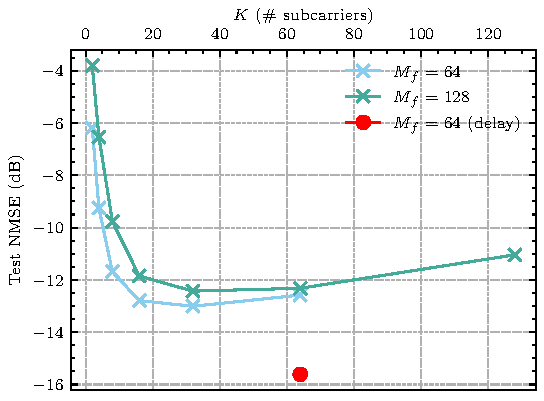
\includegraphics{outdoor_K_subc_sweep.pdf}
    \caption{NMSE vs. $K$ subcarriers of shared model architectures (i.e., complexity is w.r.t. FLOPs and parameters at UE). Outdoor COST2100 model.}
    \label{fig:outdoor_nmse_vs_K}
\end{figure}

\begin{figure}[!hbtp]
    \centering
    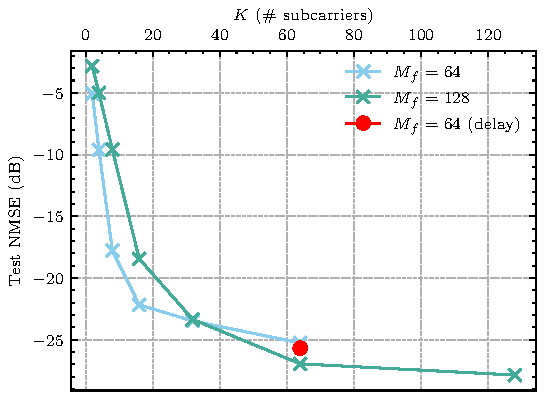
\includegraphics{indoor_K_subc_sweep.pdf}
    \caption{NMSE vs. $K$ subcarriers for shared model architectures (i.e., complexity is w.r.t. FLOPs and parameters at UE). Indoor COST2100 model.}
    \label{fig:indoor_nmse_vs_K}
\end{figure}

\subsection{Accuracy vs. Network Complexity} \label{sect:acc_vs_comp}

In Figures~\ref{fig:outdoor_nmse_vs_complexity} and~\ref{fig:indoor_nmse_vs_complexity}, we compare the reused models with frequency domain compression against the original model with delay domain compression (shown in {\color{red}red} in both Figures). Both Figures show the performance of the given model vs. a complexity metric, either log(FLOPs) or the number of model parameters. The complexity of the model varies with $K$, which we vary in the same way as described above in Section~\ref{sect:acc_vs_k}. Importantly, each complexity metric is given for the \emph{encoder} (i.e., the UE-side complexity).

\begin{figure}[!hbtp]
    \centering
    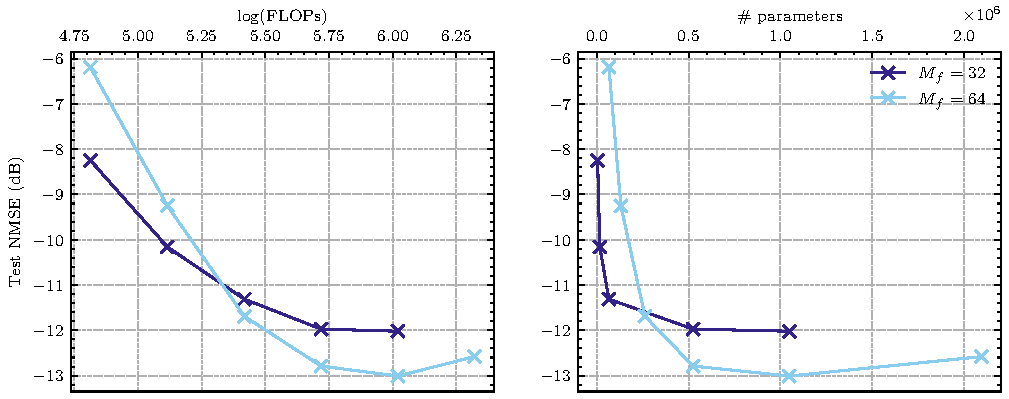
\includegraphics{outdoor_subc_sweep_line.pdf}
    \caption{NMSE vs. encoder complexity of shared model architectures (i.e., complexity is w.r.t. FLOPs and parameters at UE). Outdoor COST2100 model.}
    \label{fig:outdoor_nmse_vs_complexity}
\end{figure}

\begin{figure}[!hbtp]
    \centering
    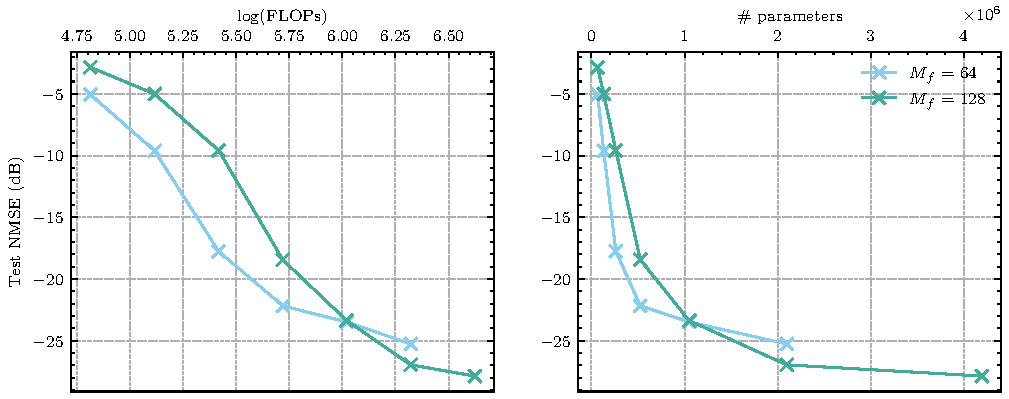
\includegraphics{indoor_subc_sweep_line.pdf}
    \caption{NMSE vs. encoder complexity for shared model architectures (i.e., complexity is w.r.t. FLOPs and parameters at UE). Indoor COST2100 model.}
    \label{fig:indoor_nmse_vs_complexity}
\end{figure}

Figures~\ref{fig:outdoor_nmse_vs_complexity_w_dec} and~\ref{fig:indoor_nmse_vs_complexity_w_dec} show the same performance and complexity metrics as Figures~\ref{fig:outdoor_nmse_vs_complexity} and~\ref{fig:indoor_nmse_vs_complexity} but with respect to the full model complexity (i.e., encoder and decoder, UE-side and BS-side). When it comes to parameters, we observe trends that are similar to the encoder-side parameters in both environments. However, the number of FLOPs for the $M_f=128$ case is twice that of the the $M_f=64$ case since the number of FLOPs of the decoder scales linearly with $M_f$.

\begin{figure}[!hbtp]
    \centering
    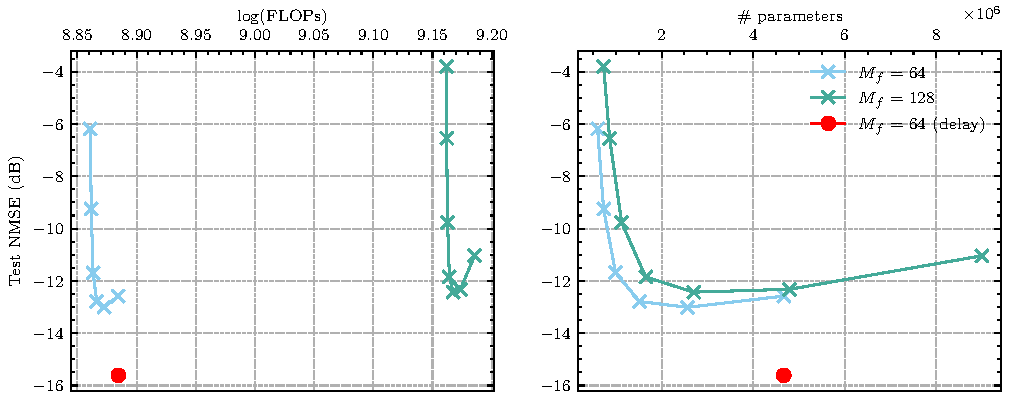
\includegraphics{outdoor_subc_sweep_line_w_dec.pdf}
    \caption{NMSE vs. complexity of shared model architectures. \textbf{Left}: Complexity w.r.t. FLOPs of encoder and decoder. \textbf{Right}: Complexity w.r.t. parameters of encoder and decoder.). Outdoor COST2100 model.}
    \label{fig:outdoor_nmse_vs_complexity_w_dec}
\end{figure}

\begin{figure}[!hbtp]
    \centering
    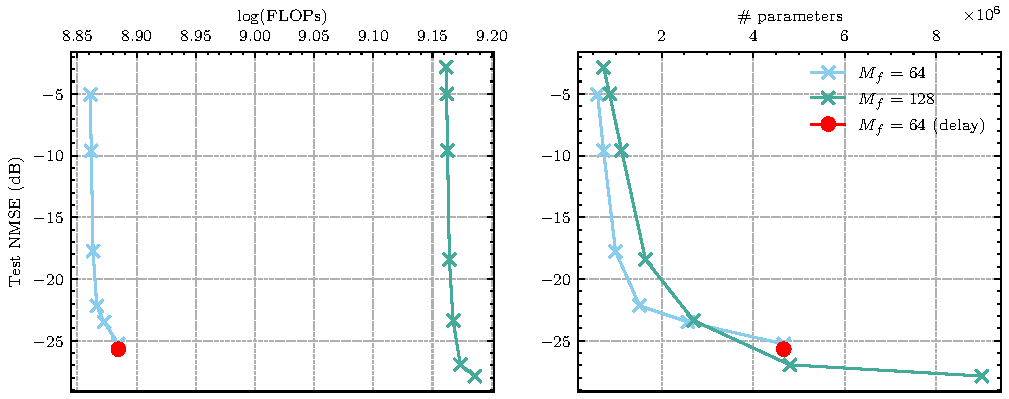
\includegraphics{indoor_subc_sweep_line_w_dec.pdf}
    \caption{NMSE vs. complexity for shared model architectures. \textbf{Left}: Complexity w.r.t. FLOPs of encoder and decoder. \textbf{Right}: Complexity w.r.t. parameters of encoder and decoder.). Indoor COST2100 model.}
    \label{fig:indoor_nmse_vs_complexity_w_dec}
\end{figure}

\section{Discussion}

In this chapter, we presented two methods for reducing the complexity of deep learning based CSI compression networks. We first proposed to move the delay domain estimation to the BS by compressing and feeding back frequency domain information to directly estimate the pilots at the UE. We then proposed to use a deep learning model to estimate blocks of $K$ contiguous subcarriers. We tested a combination of both of these approaches in both the Indoor and Outdoor COST2100 scenarios, and we demonstrated that these approaches can reduce the UE-side computational complexity while maintaining or slightly increasing the network's final accuracy.